68. a) $f(x)=x^2-2|x|=\begin{cases}x^2-2x,\ x\geqslant0,\\ x^2+2x,\ x<0.\end{cases}$
$$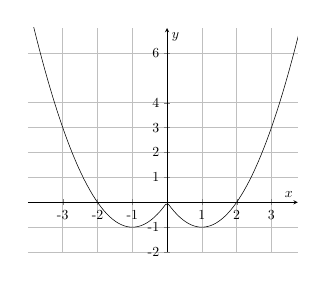
\begin{tikzpicture}[scale=0.5]
\begin{axis}[
    axis lines = middle,
    grid=major,
    legend pos={south west},
    xlabel = {$x$},
    ylabel = {$y$},
    ymin=-2,
    ymax=7,
    xmin=-4,
    xtick={-3,-1,1,3,5,2,-2,4,6},
    xticklabels={-3,-1,1,3,5,2,-2,4,6},
    ytick={ -1,6, 2,-6, -2,1,4,-4,3,-3,12},
    yticklabels={-1, 6, 2,-6, -2,1,4,-4,3,-3,12}           ]
	\addplot[domain=-4:4, samples=100, color=black] {x*x-2*abs(x)};
%\addplot[domain=-3:5, samples=100, color=black] {-abs(x-1)};
%\addplot[domain=-3.1:2.5, samples=100, color=red] {70*abs(1-2*abs(abs(x)-2))-10*x^2+10*x-70};
	%\addlegendentry{$\text{Рис. 1}$};
\end{axis}
\end{tikzpicture}$$
b) Исходя из графика, найдём ответ $a=0.$\\
